\chapter{Algorithms for mtDNA Classification to Haplogroups}
\label{chapterHaplogrep}
Human mitochondrial DNA being a non-recombinant DNA, is strictly inherited maternally. Mutations which occur over the time and get fixed mutations by passing on to the next generation, undergo a so called positive selection. Negative selection imposes the ending of a germline. So, in theory, if no mutations would occur on the mitochondrial genome, all eukaryotes from the first "mitochondrial Eve" or often also referred to as Most Recent Common Ancestor (MRCA) to the current living human beings, all should carry the same mtDNA sequences. However over the time, mutations accumulated (and still do), which are passed on to the following generations, rendering it possible to reconstruct a tree of life. This is not only affecting humans, but all eukaryotic beings (including the 4 kingdoms Plantae (plants), Fungi ,Protista (unicellular organisms) and Animalia including homo sapiens). The mutation rate of the human mtDNA is much higher than the one for the nuclear DNA with an substitution rate of 1.665 x $10^{-8}$ ($\pm$ 1.479 x $10^{-9}$) per base per year or one mutation every 3,624 years to get a fixed mutation \cite{Soares2009}. This makes mtDNA an ideal tool for reconstructing the human ancestry by confirming the out of Africa theory and helping to understand the colonization of humans over the time on the various continents. The branches of this phylogeny or tree are called haplogroups, comprising a collection of related individuals with their mutually shared mitochondrial haplotypes \cite{Scally2012}. \\
Knowing the mtDNA haplogroup affiliation is a critical prerequisite \cite{Kloss-Brandstatter2011} for studying mechanisms of human evolution and discovering genes involved in complex diseases. Besides these applications, validating phylogenetic consistency using haplogroup classification gains importance in quality control. Despite the availability of Phylotree \cite{VanOven2009}, a regularly updated classification tree of global mtDNA variation, the process of haplogroup classification was time-consuming and error-prone, as researchers had to manually compare the polymorphisms found in a population sample to those summarized in Phylotree, polymorphism by polymorphism, sample by sample. To circumvent these limitations, this chapter provides a solution to the problem of haplogroup classification based on given mitochondrial DNA profiles. The application called HaploGrep presents a fast, reliable and straight-forward algorithm and is implemented as a freely accessible Web application. The presented method is able to determine the haplogroup affiliation of thousands of mtDNA profiles within seconds, otherwise cumbersome compiled by hand. The input profiles can represent the whole mitochondrial genome, or any part of it from sequencing projects, as well as just specific genotypes information as derived with of microarrays or genotyping platforms. HaploGrep is based on the latest version of Phylotree (currently Version 17) by offering scientists in various areas (i.e. clinical genetics, population genetics, archeoegenetics or forensics) an all-in-one solution for quality assessment of mtDNA profiles, with high accurate haplogroup results. \\
This chapter starts with an overview on the different tools currently available for the haplogroup classification of mitochondrial genomes\ref{hg:related}, provides insights in the methods and algorithms implemented in the presented solution HaploGrep\ref{hg:haplogrep} by comparing its performance with tools from the related work section. Further different alternative algorithms are presented and the dissimilarity distances \ref{hg:dissimilarity} are also compared regarding run-time and accuracy. An important aspect of the analysis of mitochondrial genomes with the phylogenetic information provided by Phylotree on hand, is the feature of quality control \ref{hg:qc}. For instance, if a sample shows mutations belonging to two different haplogroups, this could indicate artificial recombination in the lab. There are several other possible sources of contamination, sample swap or contamination, that can be located based on phylogenetic trees. This chapter ends with a conclusion\ref{hg:outlook} and gives an outlook on the features for a future update.  
\section{Related Work}\label{hg:related}
When we first described our haplogroup classification approach in 2010\cite{Kloss-Brandstatter2011}, only few automatic approaches for haplogroup classification where present. By then we ware aware two tools both showing some weaknesses, that were presented in our paper: mtDNAmanager \cite{Lee2008}  and MitoVariome \cite{Lee2009}. Since there was an obvious demand for such tools, several new approaches were published thereafter. Table \ref{table:tools} gives an overview of the automated mtDNA haplogrouping methods available as of October 2016. As can be seen, there's still a huge interest of the mtDNA community to improve the haplogrouping tools. This chapter provides information on both HaploGrep as well as the updated version HaploGrep 2 in Section \ref{hg:haplogrep}.

\begin{table}
  \begin{tabular}{lllll}
    \toprule
    Method  & Year &  Reference & Cited $^*$\\ 
		\midrule
		mtDNAmanager & 2008 & Lee et al. \cite{Lee2008} & 61\\ 
		MitoVariome & 2009  & Lee et al. \cite{Lee2009} & 12\\
		mtPhyl & 2009 &  Eltsov and Volodko \cite{eltsov2009mtphyl} & \\
		Ensemble Learning & 2010 &  Wong et al,. \cite{Wong2011} & 11  \\ 
		\textbf{HaploGrep} & \textbf{2010} & \textbf{Kloss-Brandst{\"a}tter et al.}\cite{Kloss-Brandstatter2011} & \textbf{244}  \\ 
		mthap & 2010 & Lick&\\ 
		MitoTool & 2011 & Fan and Yao \cite{Fan2011} & 74\\
		HaploSearch & 2011 & Fregel et al. \cite{Fregel2011}  & 12 \\
		HmtDB: mt-classifier & 2012 & Rubino et al., \cite{Rubino2012}& 61 \\
		mtdnacommunity & 2012 & Behar et al. \cite{Behar2012} (RSRS) & 236\\
		mtDNAoffice & 2012 & Soares et al. \cite{Soares2012} & 2 \\
		EMMA & 2013 & Roeck et al. \cite{Rock2013} & 37\\
		Updated MitoTool& 2013& Fan and Yao \cite{Fan2013} & 35\\
		HaploFind & 2013 & Vianello et al. \cite{Vianello2013} & 33\\
		Phy-Mer & 2014 & Navarro-Gomez et al. \cite{Navarro-gomez2014} & 7\\
		\textbf{HaploGrep 2} & \textbf{2016} & \textbf{Weissensteiner et al.} \cite{Weissensteiner2016a}  & \textbf{14}\\

		\bottomrule
\end{tabular}
\caption[Related work]{Overview of automated haplogrouping tools for human mtDNA, $^*$number of citations as of March, 2017 in Google Scholar\footnote{\url{https://scholar.google.com/}}}
\label{table:tools}
\end{table}

Thereby different methods for the haplogroup classifications are applied by the various approaches. \textbf{mtDNAmanager} used algorithms based on propositional logic via hierarchival verification, without further specifiying the algorithm in detail. On a pre-determined list of control region mutation motifs which are stored in a MySQL database, a query system accepts the classification requests and returns the most-probable mtDNA haplogroup based on 9,294 control region sequences. The match probability is estimated by the frequency of a haplotype by $(x+2)/(n+2)$ according to Balding and Nichols\cite{Balding1994}, where $x$ is the number of times a haplotype appears in the database of size $n$. A limitation is however the use of the mtDNA control region only (16024–16569; 1–576), being often to coarse for an exact haplogroup classification.\\
\\
\textbf{Mitovariome} by Lee et al,. \cite{Lee2009} was another database of precalculated sequences, allowing to query for polymorphism, haplogroups and genbank Accession numbers. However it wasn't mantained further and is not available anymore.\\
\\
\textbf{mtPhyl}\label{mtphyl} which was not published in a journal, but only presented at the ASHG meeting in 2008 presents one of the most unknown but most influencing tool in the field of haplogrouping. It applies a maximum parsimony-based method for reconstructing the mtDNA phylogeny, estimates the mitochondrial haplotype and calculates the coalescence time of clusters. Based on the phylgenetic reconstruction by this tool, the current human mitochondrial phylogeny represented by Phylotree was enabled which is still subject to a continuous update process\cite{VanOven2015}. mtPhyl can be downloaded from \url{https://sites.google.com/site/mtphyl/home}\\ 
\\
A completely different approach for haplogroup estimation was presented by Wong et al.\cite{Wong2011} By the use of two different \textbf{machine learning approaches}, the limitations of earlier used nearest-neighbor methods were tried to solve. Based on Principal Component Analysis (PCA) and the\textbf{ Random Forest} (RF) algorithm (being an ensemble learning algorithm) haplogrouping was performed. The second method presented was a \textbf{Support Vector Machine} (SVM) algorithm. Both methods are requiring training data sets. The overall macro-accuracy of the two methods were 87.35\% and 88.06\% respectively, indicating problems with some particular haplogroups (especially haplogroup R* and N*, with a macro-accuracy of $\sim$ 10\% and 49.21\% for RF and 11.67\% and 52.38\% respectively). \\
\\
\textbf{mthap} was developed since 2010 on private initiative of James Lick and adresses data input for single samples. It is not intended for academic purpose but helps individuals interpreting their data from direct-to-consumer personal genome tests (for example 23andMe\footnote{\url{23andme.com}} data).\\
\\
\textbf{MitoTool} was published in 2011 and got updated in 2013. It comes with an own database with currently 22,525 mtDNA sequences according to Phylotree 15 and allows detailed parsing and annotation of fasta and variants input data. It is suitable for both, rCRS and RSRS references, and allows the transformation of a fasta-like format to each other. The updated version comes with a stand-alone version, which is often required for complying with data privacy laws, especially in the field of forensics and clinical research. The similarity parameter $S$ is calculated for each haplogroup where $S=2M-N$ for $M$ representing the number of shared variants between query and tested haplogroup and $N$ being the number of all variants required by the currently tested haplogroup. The complexity is thereby $O(n)$.\\
\\ 
\textbf{HaploSearch} was designed to get the variants from a multiple-alignment format fasta file or to generate multiple-alignment fasta sequences from variants (for example from, by requiring a reference sequence. This way it is more flexible and can be used also for non-mtDNA data. HaploSearch determines the haplotype, but no classification to haplogroups is provided.\\
\\
The human mitochondrial genomic resource HmtDB provided its haplogroup prediction tool \textbf{fragment-haplo-classifier} in 2012 which later was updated to the \textbf{mt-classifier}tool as part of the MToolBox pipeline. It is python based and relies on the RSRS reference. It allows the classification of haplogroups based on Phylotree, by accepting fasta files which are aligned by using Muscle. The distance measurement is similar to MitoTool, where variants from the query sequence are mapped to haplogroups predefined in Phylotree (referred to as $N_{ph}$) are set in relation to the expected number over the the corresponding region (denoted as $Nph_{exp}$), resulting to the prediction percentage per haplogroup $P_{Hg}=N_{ph}/Nph_{exp}$, where only values $>90\%$ are emitted as results.\\
\\
In 2012 the discussion about the human mitochondrial genome reference sequence got a new attention. Behar et al introduced the Reconstructed Sapiens Reference Sequence (RSRS) as a "`Copernican"' reassessment of the human mtDNA phylogeny. While there are good reasons to this change-over, it can lead to additional confusion especially in the forensics and clinical research \cite{Bandelt2013}. The presented online appearance \url{http://www.mtdnacommunity.org} provides tools for transformation (FASTmtDNA) as well as haplogroup labeling and phylogeny-based quality control with \textbf{mtDNAble}. The method behind mtDNAble was however not described.\\
\\
With \textbf{mtDNAoffice}, Soares et al. \cite{Soares2012}, present a human mtDNA macro haplgroup assignment tool for the protein coding region of the mitochondrial genome. Thereby a vectorial representation method was used, by "`naturally aligning mtDNA protein-coding region"' in a first step. The resulting genetic distance matrix was used to construct neighbor-joining or an Unweighted Pair Group Method with Arithmetic Mean (UPGMA) tree. Excluding the hypervariable control region as input is however limiting the accuracy of haplogroup estimation.\\
\\
The Institute of Leval Medicine (GMI) at Innsbruck was developing \textbf{EMMA} in 2013 together with Mannis van Oven, author of Phylotree, being also involved in mtdnacommunity and Phy-Mer. Based on a combination of database and the use of Phylotree, haplogroup estimation is performed by applying a maximum likelihood ranking. Maximum-Likelihood Estimation (MLE) was applied earlier by the Genographic Consortium \cite{Rosset2008} succesfully for site-specific mutation rates in mtDNA, where only partial phylogeny was taken into consideration. After estimating the fluctuation rate per variant, the cost function in EMMA was denoted as $C_t(b) = \sum_i{c(b_i,t_i)}$ by $i$ iterating over all positions where the query ($t$) and the currently tested profile ($b$) differ, by scaling the positional costs logarithmically to  $c(b_i,t_i)= lg(r(t_i \rightarrow t_i)/r(b_i \rightarrow t_i))$. \\
\\
\textbf{HaploFind} can be seen as a HaploGrep clone for haplogrouping performed according to the RSRS as reference sequence for complete sequences. It makes use of the suffix-tree based algorithm Mummer for sequence alignment and comparison which is performing great, but needs careful handling of variants, since the nomenclature can differ to phylogenetic standards. The algorithm for haplogroup classification is based on the pre-calculated variant scores from $sim$ 7,800 samples. The assignment is processed in a  recursive manner, where query and the tested haplogroup "`are compared by searching for matches, summing to the sequence score the score of each matching variant"' \cite{Vianello2013}.\\
\\
\textbf{Phy-Mer} is the latest approach from 2014, to perform haplogroup classification directly on sequencing data, without an actual alignment by further being reference independend. It is one of the first mitochondrial haplogroup classification tools to take data from NGS devices in form of FASTQ or BAM files into account. Using a k-mer library based on Phylotree, the distances to the query sequence are calculated by comparing the sets of all possible k-mers. \\

\section{HaploGrep}\label{hg:haplogrep}
\subsection{Architecture}
HaploGrep was initially implemented as a Java application with several modules, and got extended to a Web application on a client-server architecture. The first module is the parser based on JExcelApi\footnote{\url{http://jexcelapi.sourceforge.net/}} for spreadsheet input files. Phylotree provides the clearly structured data as HTML versions for manual navigation from an Microsoft Excel sheet. We therefore re-coded the XLS file to a XML file by using the standard libraries provided by Java. For every new update of the Phylotree versions to be used with HaploGrep, three steps are required: 
\begin{enumerate}
\item preprocessing step directly incorporated in Excel which was written in Visual Basics for Application (VBA) to check for data integrity (i.e. missing lines or empty labels). 
\item the actual transformation from XLS to XML with our Parser, which runs recursively over the XLS file and writes the haplogroup name, all profiles, accession number and references if provided to the XML file. HaploGrep relies on the rCRS, hence all profiles are reported as list of nucleotide positions that deviate from this reference. 
\item The newly generated XML file is parsed for generating the fluctuation rates per position. The corresponding algorithms used can be found in the next subsection \ref{haplo:alg}.
\end{enumerate}
As mentioned, the core of HaploGrep is implemented as a java library and is structured in an own Java Package. The application was thereafter designed as a Web application based on client-server architecture. This way all the computational intensive tasks are performed on server side, by getting use of REST for the client-server communication, implemented within the Restlet Framework. For every request a server side generated session object is created and encrypted through a session key. The XML based tree is loaded once in an in-memory hash table, increasing HaploGrep's speed significantly compared to other methods (see Figure 3 in \cite{Kloss-Brandstatter2011}). We also take advantage of current multicore architectures by handling requests efficiently in concurrent ways. For this to take place, we take advantage of multi-threading by using JAVA's \verb|java.util.concurrent| packages, by using mostly \verb|ConcurrentHashMap| and \textit{worker threads} by using \textit{thread pools}, which reduce overhead due to thread creation, avoiding memory management overhead otherwise caused by allocating and deallocating many thread objects \footnote{\url{https://docs.oracle.com/javase/tutorial/essential/concurrency/pools.html}}. \\
The front-end of the client is implemented in JavaScript as HTML5-based rich internet application, by using the EXT-JS JavaScript MVC framework\footnote{\url{http://www.extjs.com}}. The communication is AJAX based, which means we use asynchronous HTTP requests, with the earlier mentioned REST-resource, by using JSON\footnote{\url{http://www.json.org}} and XML as standard exchange formats. For the graphical representation of the Phylotree, the InofVis Toolkit \footnote{\url{(http://thejit.org}} is applied. Additionally BioJava \cite{Prlic2012} and the high performance collections library Trove\footnote{\url{http://trove.starlight-systems.com/}} where used for the input of fasta sequences as presented in Chapter \ref{chapterAlignment}, which outperform JDK's collections by using open addressing for primitive types. The Htsjdk JAVA API provided by the Broad Institute \footnote{\url{https://github.com/samtools/htsjdk}} was integrated for the import of VCF (Variant Call Format) files.

\subsection{Input Data Formats}\label{hg:input}
Besides the own data input format defined in the first version of HaploGrep called \verb|*.hsd| format, HaploGrep 2 supports several new data input formats. 
The *.hsd file is a simple text file, consisting of at least 4 columns; ID for the sample identifier, the targeted mtDNA region, either as range seperated by "`-"' or single SNPs seperated by "`;"', the haplogroup if already estimated, and the polymorphisms seperated by tabs. Table \ref{table:hsd} gives an example of HaploGrep's standard input format.
The format is similar to the EMPOP format\cite{Parson2007}, with the main difference that the range can be specified directly per row.
\begin{table}[H]
  \begin{tabular}{lllllll}
    \toprule
    ID & Range & Haplogroup & SNP &  &  \\
		\midrule
	Sample1 & 16024-16569; &  & 16051G & 16051G & 16182C\\
	Sample2 & 16024-16569;1-576; &  & 16224C & 16311C & 146C\\
	... & ... & & ... & & & \\
		\bottomrule
\end{tabular}
\caption{Example of an *.hsd file, the standard input format for HaploGrep}
\label{table:hsd}
\end{table}

HaploGrep in the updated version 2 accepts further input formats, being FASTA files and VCF files. While for the fasta import there exist different implementations, one requiring an additional alignment step, the use of HTSJDK allows the direct import of VCF files. The files are parsed and converted so that the internal objects can be used, which were designed for the hsd files. The methods behind the alignment step are presented in detail in Chapter \ref{chapterAlignment}. 
\\
The structure of the VCF files was presented in the Introduction (see \ref{intro:VCF}). As short repetition, the file is tab-separated, with 8 fixed fields or columns, that are compulsory, and can be extended to the users need. The specifications can be found on the Github page\footnote{\url{https://vcftools.github.io/specs.html}}.

\subsection{Algorithm}\label{haplo:alg}
The main idea behind HaploGrep is the usage of Phylotree as database, by calculating for each variant occurring in the tree a so called phylogenetic weight. This weight is an assessment of the stability of a SNP. In the first version of HaploGrep the following method for assigning the phylogenetic weights is used: by traversing the Phylotree, for every mutation the amount of occurrence gets estimated. The SNP with the highest occurrence (m.152T$>$C occurred 106 times in Phylotree 10 used for the publication) + 1 is taken as reference value. The weight is obtained by subtracting the number of occurences from the reference value. This way SNPs with higher occurence get a lower weight than SNPs occuring only once. Hotspot Mutations like m.16519T$>$C where assigned value 0. Listing \ref{alg:haplo1} represents the weighting more formally:

\begin{algorithm}\label{hg:algorithm}
\caption{Scoring of weights in the first version of HaploGrep}
\label{alg:haplo1}
Let the index set $I$ refer to all mutations found at least once in PhyloTree, and for each $i \in I$ let $f_i$ the absolute frequency of mutation $i$ on the current build of PhyloTree. Let $F$ = $max(i_{fi})$ be the maximum of all those frequencies. For $i \in I$ put the weight $w_i = F-f_i$. 
\end{algorithm}

As an example, consider the demonstration provided in the paper\cite{Kloss-Brandstatter2011}: assume that a sample was sequenced for the entire control region (nucleotide positions 16024–16569; 1–576) and genotyped for 45 coding region SNPs as described by Brandstaetter et al. It showed the following profile (with corresponding weights): m.263A$>$G (105),m.309 - 310insC (0),m.315 - 316insC (0),m.750A$>$G (106), m.951G$>$A (103), m.8860A$>$G (106), m.15326A$>$G (106), m.16354C$>$T (101), and m.16519T$>$C (0). The polymorphisms m.309 - 310insC, m.315 - 316insC, and m.16519T$>$C were hot spots and therefore not taken into consideration (weighted with 0). For every haplogroup the rank was calculated according to HaploGrep's algorithm: haplogroup H2a1 was rated best because all diagnostic polymorphisms for the haplogroup were found in the sample $[(105+106+103+106+106+101)/(105+106+103+106+106+101) = 1]$ and none of the sample’s polymorphisms remained unexplained or private $[(105+106+103+106+106+ 101)/(105+106+103+106+106+101+0+0+0)=1]$. Therefore, the overall rank for H2a1 was $r_{H2a1}=0.5\times 1.0 + 0.5 \times 1.0 = 1.0$. For example, the third best hit was haplogroup H2a, where the value for the first part of equation was still 1.0 but because two polymorphisms (m.951G4A, m.16354C4T) remained unexplained in the sample’s profile, the second part of the equation was $(105+106+106+106)/(105+106+103+106+106+101+0+0+0) = 0.6746$, thus leading to a final rank of $r_{H2a}= 0.5\times 1.0 + 0.5\times 0.6746 =0.837$.\\
In the updated version of HaploGrep 2, this value was classified with a more sophisticated phylogenetic weight, where we scaled the weights in a window from 1 to 10. Listing \ref{alg:haplo2} shows the new phylogenetic weight.
\begin{algorithm}
\caption{Scoring of weights in the new version of HaploGrep 2}
\label{alg:haplo2}
Let the index set $I$ refer to all mutations found at least once in PhyloTree, and for each $i \in I$ let $f_i$ the absolute frequency of mutation $i$ on the current build of PhyloTree. Let $F$ = $max(i_{fi})$ be the maximum of all those frequencies. For $i \in I$ put $w_i = 1+(9/\ln(F)) \times [\ln(F) - \ln(f_i)] = 10-9\ln(f_i) / \ln(F)$. Conversely, given $1 \leq w \leq 10$, the corresponding frequency $f$ is calculated as  $f = F(10 - w)/9$.
\end{algorithm}

Based on the calculated weights per variant $w_i$ we calculate for every haplogroup in phylotree the distance to the query variants $r_{hg}$, where we take into account how often variants are found per haplogroup ($k$), the number of variants expected in the analyzed range of the tested haplogroup ($m$) and the total number of polymorphisms in the query sample ($k$).

\begin{equation}
	r_{hg} = \frac{1}{2} \times \left(\frac{\sum^{k}_{i=1} w_i}{\sum^{m}_{i=1} w_i} + \frac{\sum^{k}_{i=1} w_i}{\sum^{n}_{i=1} w_i}\right)
\end{equation}

Thereby the formula shows that this rank is composed of two parts. The first component calculates the weighted ratio of haplogroup-associated polymorphisms that were found in the sample to the total number of haplogroup-associated polymorphisms in the currently tested haplogroup within the analyzed range. The second part reflects the ratio of polymorphisms in the test sample that are associated with the haplogroup under investigation to the total number of polymorphisms found in the test sample. This second component assures that a result will be ranked higher if it uses as many polymorphisms in the sample as possible. The two components are weighted equally and form the final overall rank $r_hg$. The resulting list is sorted according to these ranks to present the user the best results first. When we first described this algorithm, we were'nt aware that this formula was described by Stanisław Kulczyński in 1927. The Kulczynski similarity 2 is a similarity for numerical data in $\mathbb{R}^n$, according to \cite{Deza2009}:
 
\begin{equation}
\frac{n}{2}\left(\frac{1}{\overline x}+\frac{1}{\overline y}\right) \sum{min(x_i, y_i)}
\end{equation}

where $x$ and $y$ represent non-zero vectors ($x=(x_1,...,x_n)$ and $y=(y_1,...,y_n)$). $\overline x$ denotes $\frac{\sum{x_i}}{n}$ corresponding to the \textit{mean value} of components $x$. Same holds true for $\overline y$. $n$ is the length of the vectors.

Since we parse the Phylotree as a structured XML tree in memory, by loading it once, queries are handled in a recursive manner. Listing XX represents the pseudo-code for the calculation of the ranks where $max(r_{hg})$ represents the best hit.

\begin{lstlisting}
searchPhylotree(Node, Result[], sample, parentResult){
 childrenNodes[] = PhyloTreeNode.getSubHaplogroups();
 while(childrenNodes.hasMoreElements) {
  SearchResult result = new SearchResult(childrenNodes, parentResult);
  List polys = childrenNodes.getExpectedPolys();
   while (polys.hasMoreElements) {
    if (testsample.contains(currentPoly)) {
      if (!currentPoly.isBackMutation()) {
        if (newResult.contains(currentPoly)==1) {
          newResult.addExpectedPolyWeight(poly);
          newResult.addFoundPolyWeight(poly); }
        else {
          if (currentPoly.isBackMutation()) {
            newResult.removeMissingOutOfRangeWeight(currentPoly);}
            newResult.addExpectedPolyWeight(currentPoly);}
      }
    }
     else
       newResult.addMissingOutOfRangeWeight(currentPoly);
   }
  results.add(newResult);
  searchPhylotree(currentElement, results, sample, newResult);
}
\end{lstlisting}

\subsection{Output formats}

The main concept of HaploGrep, is to provide all relevant data immediately in the browser, after the haplogroup classification is performed automatically after the file upload. Also the file-exports are represented in a graphical way in the browser prior the download by the user. Several new browser- and file-based outputs can be generated:
\begin{enumerate}
\item Haplogroups Report: all the data generated for the haplogroup classification are summarized in a table. The information provided comprises the resulting haplogroup per sample, with its quality score (default Kulzczynski-distance)). Further the remaining polymorphisms not assigned, the polymorphisms not found in the top ranked haplogroup are listed, as well as the annotation of the corresponding amino acid changes provided in Pereira et al \cite{Pereira2011} and the input profile.
\item Multiple Alignment Format: based on the rCRS reference sequence, HaploGrep provides a multiple sequence alignment format. This format aligns all sequences to the same length, by extending it for insertions if present. Deletions are denoted with "-" and handled identical to base substitutions. This way a cost intensive multiple sequence alignment is reduced to a pairwise alignment, with an additional help of a vector storing the indels. The details can be found in Chapter \ref{chapterAlignment}. The  generated multiple sequence alignment in fasta format and can be directly viewed in the browser, based on the implemented BioJS open source JavaScript framework for biological data visualization \cite{Gomez2013}. Having the multiple alignment format at hand, the freely available tool PGDSpider \cite{Lischer2012} can be used subsequently for downstream analysis, by converting the result into a variety of population genetics formats. Some of the gold standard tools supported this way are ARLEQUIN (21), MEGA (39), 
MIGRATE (40), PHYLIP (41) directly or the NEXUS format (42) for MRBAYES(23) or PAUP*(22).
\item VCF: a column-based representation of all samples, as described in the section Input formats \ref{hg:input} is generated based on the HTSJDK Java library. The VCF file is also represented in the Browser, by ignoring the VCF header and only showing the data lines represented in a table for better human readability. The VCF file including the header can be downloaded for further analysis such as the Fixation index ($F_{ST}$) computation, linkage disequilibrium (LD) association, or Principal Component Analysis (PCA), by the freely available VCFtools \cite{Danecek2011} directly or to generate PED and MAP files for further analysis with the toolset PLINK \cite{Purcell2007}.
\item  FASTA: each sample is exported as sequence entry in one summarizing fasta file, excluding the alignment in- formation.
\item Phylogenetic Tree: as additional graphical representation, the estimated haplogroups can be represented as a Phylogenetic tree, which for many researchers is an attractive feature, as it represents how classified haplogroup results fit into the existing phylogeny, based on Phylotree. All classified samples are combined to a resulting rooted tree, that incorporates all polymorphisms relative to the rCRS. The user can further customizing the output by selecting whether hot spot mutations should be taken into account and the export format used. The generated tree can be directly be opened in the browser or downloaded in one of the fomrats: either as pdf, svg or png file. The vector graphic formats (pdf and svg) can thereafter be modified in any vector graphics software like Inkscape\footnote{freely available at \url{https://inkscape.org/}}. The output format is implemented by using the Apache Batik SVG Toolkit \footnote{\url{https://xmlgraphics.apache.org/batik/}}. Figure \ref{hg:phylogeneticTree} provides an example tree from the 1000G phase 3 data, classified under the haplogroup branch D4.
\begin{figure}[!ht]
    \centering
    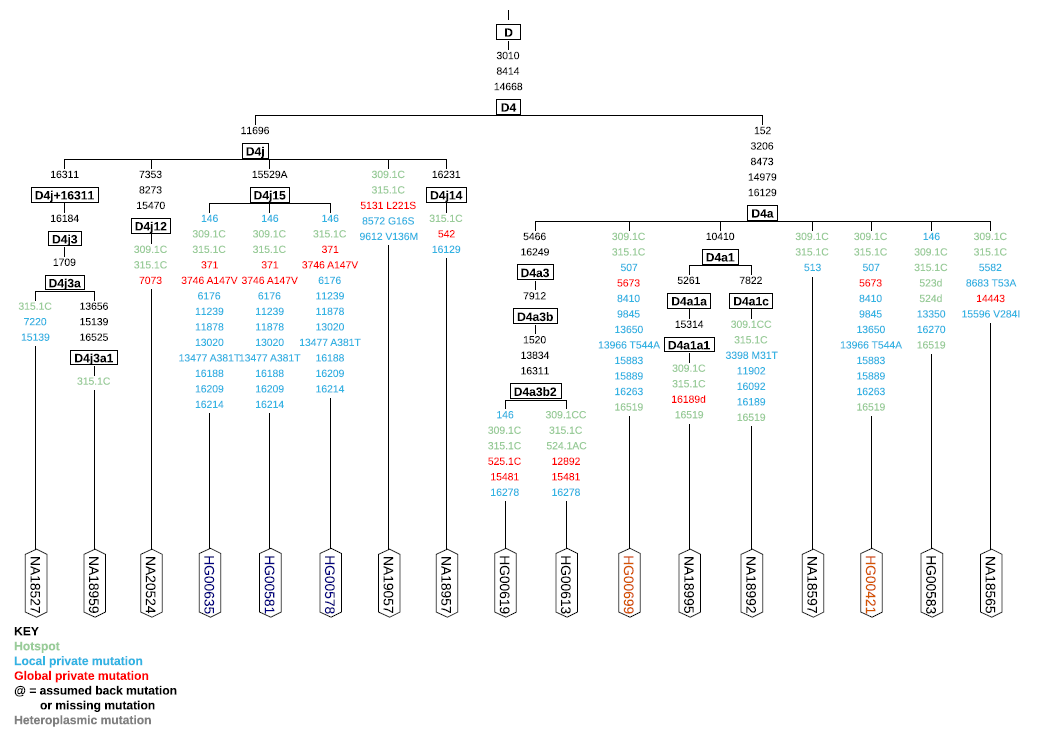
\includegraphics[width=1\textwidth]{images/tree.png}
    \caption[Export of Graphical Phylogenetic Tree]{Polymorphisms in the tips of the phylogeny are candidates for newhaplogroups, see for instance the samples belonging to haplogroup D4j15, (confirmed to be related (ftp://ftp.1000genomes.ebi.ac.uk/ vol1/ftp/technical/working/20130606 sample info/20130606 sample info.xlsx)) or samples HG00699 and HG00421 (not related). Polymorphisms marked in red are not occurring in Phylotree and may require additional attention, whereas mutations in blue are private polymorphisms for this group, already known by Phylotree. The annotation of amino acid changes and mutational hotspots (green) can be defined by the user, thereby hotspots at positions 16182, 16183 and 16519, AC insertion and deletions at 515–524, inserts at 16193 as well as variation around position 310 and point heteroplasmies can be excluded for the phylogenetic reconstruction. } 
    \label{hg:phylogeneticTree}
\end{figure}
\end{enumerate}

\subsection{Validation}
Since the aim of HaploGrep is to replace a manual process, the results are straight forward to validate. For this purpose, several measurements were taken into account: manually assigned haplogroups from different published studies (see section "Validation Using Predetermined data" in the HaploGrep paper \cite{Kloss-Brandstatter2011}), were reassigned with HaploGrep and checked for concordance. This process was automated by using the unit testing framework JUnit \footnote{\url{http://junit.org/}}. Thereby these tests validate if HaploGrep results in the expected predetermined haplogroups. These tests are performed with every HaploGrep update. We further compiled a dataset of 120 selected sequences covering the main branches of the human mitochondrial phylogeny (see HaploGrep paper) for test purpose to users, to see the functionality of HaploGrep, without the need of uploading own data. We further checked with the data provided in Bandelt et al. \cite{Bandelt2012} Table2 and Table3 for the correctness of the haplogroup classification. While the first data set comprises 28 selected control region profiles or partial HVS-I and HVS-II sequence range, the latter represents a dataset of artificially recombined profiles, that should be detected as such. The results of this validation can be found under the section Quality Control \ref{hg:qc}.

Additionally the publicly available datasets from the 1000 Genomes Project (1000G) Phase 1 with 1,092 samples and Phase 3 comprising 2,534 samples were used for validation purpose of the different dissimilarity indices, implemented in HaploGrep 2. The provided information from the consortium are VCF files from both datasets, as well as consensus sequences in FASTA format. The results of the validation are reported in subsection \ref{subs:evaluation}. 

\section{Dissimilarity Indices for mtDNA data}\label{hg:dissimilarity}
\label{subs:distance}
The aim of HaploGrep is to get the best hit from a provided sequence or profile, by comparing it to entries in an in-memory database. Thereby the efficient distance computation is generally an important task in phylogenetics. Knowledge about the mitochondrial phylogeny needs to be taken into account, which limits the usage of ordinary distances. However distance metrics can often be applied in different scientific areas, as pointed out in the Encyclopedia of Distances \cite{Deza2009}, as example the Levenstein metric (or edit distance, Hamming+Gap metric) estimating the costs between strings. Therefore several different dissimilarity indices were taken into account for performance comparison regarding accuracy and speed. This section presents the Weighted Hamming distance, provides the introduced Kulczynksi distance for comparison with the Jaccard Indice. The Kimura 2 parameter distance differs in that the information about the substitution rates are weighted based on transition and transversion. This differs from the Jukes and Cantor's model, which assumes independent change with equal probability at all sites. Listed below are the different dissimilarity indices as applied in Haplogrep 2.

\subsection{Weighted Hamming distance}
\label{hamming}
The Hamming distance according Richard Hamming in 1950 adapted here represents the difference between two haplogroups Q and H, where Q is the group of mtSNPs to query and H represents the set of mtSNPs of a Haplogroup being an element of the Phylotree (P). Since both strings are aligned to a shared reference sequence R, the length is directly comparable in a compressed bitmask, where shared elements equal to the reference sequence can be ignored. More formally, the Hamming distance between two haplogroups Q and H is $d_H$ =  $\sum\left|Q_i-H_i\right|$ for all mtSNPs $_i$. The $\min$ $d_H$ $\in$ P represents the best haplogroup match. In order to reflect the human phylogeny, the weighted Hamming distance $d_{Hw}$ is calculated upon the phylogenetic weights presented earlier, instead of the binary mask.
Example: Assume query profile Q = (152C, 263G, 750G, 8860G, 16519) and Haplogroup H2 $\in$ P (263G, 750G, 1438G, 4769G, 8860G, 15326G) are compared. 16519 is a mutational hotspot and has weight 0, and is therefore not considered. The resulting Bitmask Q = 11100101 and H2 = 0111110 yields to 
\begin{verbatim}
Q = 152C, 263G, 750G,               8860G,        ->  1110010
H2=       263G, 750G, 1438G, 4769G, 8860G, 15326G ->  0111111
                                                      *  ** *
\end{verbatim}

$d_{H}$ distance 4. Replaced with the phylogenetic weights, the difference $d_{Hw}$ is $|1-0|+|8.8-8.8|+|10-10|+|0-10|+|0-8.8|+|10-10|+|0-10|$ = 29.8 where 10 represents the weight of a mutation with no fluctuation (for mtSNPs 750G, 1438G, 8860G and 15326G), 8.8 represents the weight of two occurrences in P (for mtSNPs 263G and 4769G) and 1 (152C) represents the highest fluctuation rate in P. Therefore this score reflects the phylogenetic distance better than simple counting of differences.

\subsection{Kulczynski Distance}
This distance is the default one applied since the first release of HaploGrep. The details are reported in Section \ref{hg:algorithm}. In order to compare this distance with the Jaccard Index, we here report the same notation, according the sets of mitochondrial profiles $A$, being a subset of all possible base substitutions $P = \left\{ p_1, p_2, ..., p_l \right\} $ with $l$ being the length of the mitochondrial genome, i.e. $l$ = 16569. 
\begin{equation}
d_k (A_1, A_2) = 1 - \frac{1}{2} \left( \frac{\left|A_1  \cap A_2\right| }{\left|A_1  \right|} + \frac{\left|A_1  \cap A_2\right| }{\left|A_2 \right| } \right).
\end{equation}
Again, take the previous example by assuming query profile $A_1$ = (152C, 263G, 750G, 8860G, 16519) and $A_2$ =  (263G, 750G, 1438G, 4769G, 8860G, 15326G) are compared. Again, we replace the polymorphisms with the phylogenetic weight estimated previously and perform the calculation. 16519 is a mutational hotspot and has weight 0.

$d_k$ = 1 - $\frac{1}{2} \left(  \frac{\left| 263G, 750G, 8880G \right|}{\left| 152C, 263G, 750G, 8860G, 16519 \right|} +\frac{\left| 263G, 750G, 8880G \right|}{\left| 263G, 750G, 1438G, 4769G, 8860G, 15326G \right|} \right)$ 
\\= 1 - $\frac{1}{2} \left(  \frac{3}{5} +\frac{3}{6} \right)$ = 0.45

by inserting the weights:
\\= 1 - $\frac{1}{2} \left(  \frac{\left| 8.8 + 10 +10 \right|}{\left| 1 + 8.8 + 10 +10 +0 \right|} +\frac{\left| 8.8 + 10 + 10 \right|}{\left| 8.8 + 10 + 10 + 8.8+ 10 +10 \right|} \right)$ 
\\= 1 - $\frac{1}{2} \left(  \frac{28.8}{29.8} +\frac{28.8}{57.6} \right)$ = 0.266\\
\begin{figure}[!ht]
    \centering
    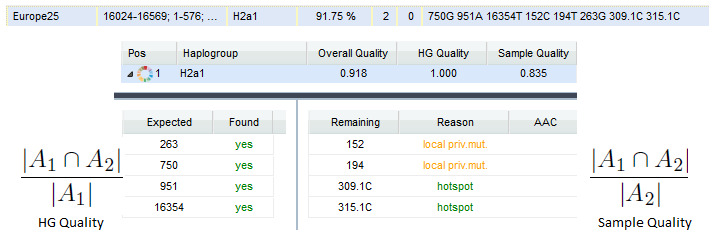
\includegraphics[width=1\textwidth]{images/HG-sample-qual.png}
    \caption[Algorithm's graphical representation in HaploGrep]{ Algorithm's graphical representation in HaploGrep} 
    \label{hg:kulczy}
\end{figure}

What can be seen here, is that the phylogenetic weights yield to a smaller discordance, rendering the two compared haplogroups more similar. The HaploGrep user interface does provide the user the information from both parts of the equation (see figure \ref{hg:kulczy}), by representing the Haplogroup quality (HG Quality) and the Sample Quality separately as scores, and by listing the polymorphisms in two tabs: expected (all $A_1$ polymorphisms are listed here, with the status found (yes, no)) and the remaining polymorphisms with the status Reason (local private mutation, global private mutation, hotspot or out of range). While out of range, hotspot and global private mutation do not influence the Sample Quality (weight 0), the local private mutation (the mutation has a phylogenetic weight and is observed in other haplogroups)  
Values are in the range between $d_k \geq 0 $ $ \wedge \leq 1$, where $1$ indicates a perfect match in HaploGrep, by not considering the $1-$ in the equation. 

\subsection{Jaccard Index}
According Henning et al \cite{Hennig2006}, the Jaccard coefficient \cite{Jaccard1901} is presumably the most widely used dissimilarity measure in biogeography. The Jaccard distance is represented by:
\begin{equation}
d_j (A_1, A_2) = 1 -  \frac{\left|A_1  \cap A_2\right| }{\left|A_1 \cup A_2\right|} 
\end{equation}
where $A$ denotes the sets of mitochondrial profiles, and $A_1$, $A_2 \in A$. Again, considering the previous example, the Jaccard distance yields to the result, $d_j$ =
1 - $\left(  \frac{\left| 263G, 750G, 8880G \right|}{\left| 152C, 263G, 750G, 1438G, 4769G 8860G,15326G, 16519 \right|}  \right)$  = 
1 -  $\left(  \frac{3}{8} \right)$ = 0.625. 

By using the weights: \\
= 1 - $\left(  \frac{\left| 8.8 + 10 + 10 \right|}{\left| 1 + 8.8 + 10 + 10 + 8.8 + 10 + 10  + 0 \right|}  \right)$  = 
= 1 -  $\left(  \frac{28.8}{58.6} \right)$ = 0.509. 
\subsection{Kimura - two parameter model}
One of the most widely used evolutionary distance, i.e. a model of DNA evolution is the KimuraThe frequency matrix for a base exchange according Kimura\cite{Kimura1980} is based on the transitions (A $\leftrightarrow$ G and C $\leftrightarrow$ T) and transversions (all other base exchanges from pyrimidine to purine and vice versa). Table \ref{hg:kimuratable} indicates the base substitution as transition (denoted as $\alpha$) and transversion (denoted as $\beta$). Thereby the model assumes an equal distribution of all nucleotides ($\pi$A = $\pi$C=$\pi$G=$\pi$T=0.25 $\mathcal{N}.$). Based on the rCRS, this is however not the case for the mitochondrial genome ( $\pi$A = 0.309 $\pi$C= 0.313 $\pi$G=0.131$\pi$T=0.247)
\begin{table}[h]
\label{hg:kimuratable}
\centering
\caption{Rate matrix of the transition states of nucleotide bases: transitions ($\alpha$) and transversions ($\beta$) for the Kimura 2 parameter model.}
\label{mtDNAsource}
\begin{tabular}{lllll}
\hline
   & A&  C   &G  & T\\
\hline

A  & - & $\beta$    & $\alpha$  & $\beta$ \\
C  & $\beta$ &  -   & $\beta$  & $\alpha$ \\
G  & $\alpha$ &  $\beta$    & - & $\beta$ \\
T  & $\beta$ &  $\alpha$    & $\beta$  & - \\
\end{tabular}
\end{table}

The Kimura two parameter distance, called K80 model (based on the year of publication), is calculated by:
\begin{equation}
K80 = - \frac{1}{2} \log((1- 2p -q ) \sqrt[]{1-2q})
\end{equation}
where the two parameters $p$ and $q$ represent the proportion of sites that show transitions and transversion respectively.

In the mitochondrial DNA the occurence of a transition is 20 times more likely than a transversion (for homoplasmic SNPs \cite{Guo2012}). Based on our analysis of the 1000G Phase 3 mitochondrial genomes, this Transition/Transversion ratio $k$ can be confirmed, varying between $k=1:17$ and $k=1:30$ depending on the reference sequence. By considering only the heteroplasmic variants in 1000G phase 3, the ratio is $k=$ \textbf{1:21}. For the nuclear DNA, the Transition / Transversion ratio assumes transitional changes about four times more likely than transversional changes \cite{salemi2009the}. 


\subsection{Evaluation}
\label{subs:evaluation}

For validation purposes we applied all four presented distances to the 1000G Phase 1 data (n=1,074) as well as to the dataset provided by Li et al.\cite{Li2014}, including 2,000 exome sequencing mtDNA data from a Danish cohort. Table \ref{table:distances} presents the summary of the evaluation. The entries in the upper triangular matrix are the percentage of identical haplogroup results between the different algorithms. Haplogroups using any “+” notation with the same slot were not considered, since MitoTool is not supporting such groups (accounts for 66 to 69 haplogroups, depending on the HaploGrep 2 algorithm used). The detailed results are provided in Supplemental Material of the HaploGrep 2 publication\footnote{\url{http://nar.oxfordjournals.org/content/suppl/2016/04/15/gkw233.DC1/HaploGrep2-SupplementalMaterial.pdf}}. 
\begin{table}[H]
\centering
\label{table:distances}
\begin{tabular}{lllll}
\cellcolor[HTML]{FFFFFF} & \cellcolor[HTML]{FFFFFF}Hamming & \cellcolor[HTML]{FFFFFF}Kulczynski & Jaccard & Kimura2P \\
MitoTool & \multicolumn{1}{c}{\cellcolor[HTML]{96FFFB}96.84} & \multicolumn{1}{c}{\cellcolor[HTML]{96FFFB}96.65} & \cellcolor[HTML]{96FFFB}96.75 & \cellcolor[HTML]{96FFFB}96.75 \\
Hamming & \multicolumn{1}{c}{\cellcolor[HTML]{FFFFFF}{\color[HTML]{330001} }} & \multicolumn{1}{c}{\cellcolor[HTML]{A9D0FF}98.98} & \cellcolor[HTML]{34CDF9}99.54 & \cellcolor[HTML]{ECF4FF}95.82 \\
Kulczynski & & \cellcolor[HTML]{FFFFFF} & \cellcolor[HTML]{A9D0FF}98.88 & \cellcolor[HTML]{96FFFB}96.28 \\
Jaccard & & & & \cellcolor[HTML]{ECF4FF}95.72 \\
\end{tabular}
\caption{Comparison of MitoTool and HaploGrep 2 with the extended dissimilarity indices in regard of the 1000G phase 1 data (n=1,076).}
\end{table}
While the run-time of the first three distances was almost identical (see table \ref{table:speed} for details) with 4.6 – 4.7 sec, the Kimura2P distance showed a 33-fold higher wall-time (158.1 sec). The ratio was similar for the Li data
(6.4 sec for Kulczynksi vs. 210 sec for Kimura2P). With the different results in 21 out of the 1,074
samples (1.96\%) in the 1000G phase 1 data, 153 out of 2,534 (6.11\%) in the 1000G phase 3 data
and 98 (4.9\%) out of 2,000 in the exome sequencing samples, the user gets additional informations
about the data quality and can check the corresponding samples. Thereby coverage problems in the
exome data and problems with the VCF file in the 1000G phase 3 data become visible (see Table 1
and Supplemental Material Table 2 - 4). We therefore provide this combined haplogroup estimation
mode (Button “Haplogroup Discordance Check”), which lists all samples where at least one metric
yields a different result.

\begin{table}[H]
\centering
\label{table:speed}
\begin{tabular}{|l|l|l|l|l|l|}
\hline
              & MitoTool  & Hamming  & Kulczynski & Jaccard  & Kimura2P   \\ \hline
1000G phase 1$^{1}$ & 177.3 sec & 4.7 sec  & 4.6 sec    & 4.7 sec  & 158.1 sec  \\ \hline
Danish Cohort$^{2}$ & 447.6 sec & 6.42 sec & 6.37 sec   & 6.39 sec & 210.97 sec \\ \hline
\end{tabular}
\caption{Wall time of haplogrouping classification over different methods, on 1,074$^{1}$ and 2,000$^{2}$ samples in form of hsd variant files - no sequence alignment required. }
\end{table}



\section{Quality Control}\label{hg:qc}
\subsection{Artificial recombination detection}
The 16,6 kilobases of the mitochondrial DNA are chopped in smaller fragments when sequenced for being amplificated with the polymerase chain reaction (PCR). This means that different fragments of one sample are sequenced. For the whole mitochondrial genome, at least 2 such fragments are needed, each comprising between 8kb and 10kb. Different protocols exist, which use 3 or more fragments. Since several manual steps are required when handling the sample in the lab, a fragment could be switched between samples - resulting in so called artificial recombination. Figure xx shows issues with fragments in an NGS sequencing project where the wrong amplification of fragments was applied due to switched concentration in the sample preparation step.
To check for issues with fragments, derived from different samples, a module "`Check for Recombination"' was implemented in HaploGrep. The algorithm for this procedure can be drafted in the following manner, on a per sample basis:
\begin{itemize}
	\item[a)] Estimate the haplogroup $H$ of the complete provided mitochondrial profile 
	\item[b)] split the sample profile according the fragments $F$ used, and estimate the haplogroup per fragment ($P_{f_i}$)
	\item[c)] split the reference haplogroup $H$ profile according the fragments $F$ and estimate the haplogroup per fragment ($R_{f_i}$)
	\item[d)] for each fragment compare the phylogenetic distance $\gamma_f(i)$ of the resulting haplogroup and calculate the total score $$\sum_{n=1}^{length(f)} |{\gamma_f(P_{f_i} - R_{f_i})| > 5}$$ where all samples with distances in the phylogenetic Tree surpassing five nodes are emitted as potentially recombinant.
\end{itemize}
As a second approach for detecting artificial recombination, the method described in Kong et al (distilling paper) for checking constituents in a sample mix-up was implemented. The basic concept here is to estimate the haplogroup of a sample in a first iteration, similar as in the previous described approach a). In a second iteration, all mitochondrial polymorphisms, that could not be assigned to the best resulting group are used to make up a new virtual profile. These secondary possible constituents are affiliated to haplogroups and the number of haplogroup defining constituents confirms the possible contamination. The two steps of the algorithm can be drafted as follows:
\begin{itemize}
	\item Primary Classification: Estimate the haplogroup $H$ of the complete provided mitochondrial profile. 
		\item Secondary Classification: For all mutatins $m$ not being covered for the primary classification, the haplogroup with the least difference to the rCRS is estimated. If the resulting haplogroups differs from H2a2a1 and the elements in $m$ are not phylogenetic hotspots, a warning for possible contamination is emmited.
\end{itemize}

Given the dataset in Bandelt et al \cite{Bandelt2012}, the herein described methods were assessed for reliability. In the first paper describing the haplogrouping classification these recombinations remained undetected by HaploGrep, which could be seen as a limitation. The check for remaining variants was able to detect six out of the seven cases, while the fragment-based check could reliably detect all samples as artificial recombinants. Table \ref{table:recomb} lists the results of the two methods, by extending the table provided by Bandelt et al. 


\begin{table}[H]
\centering
\label{table:recomb}
\begin{tabular}{lllll}
ID & HG Status & Exp. vs. Est. & Method 1 & Method 2\\ \midrule
USA.AFR.942 & L1b$|$C1 & C1c$|$X M31a1 & L1b$|$C1 &  M31a1$|$L1b3 \\
FRA.CAU.84 & HV0$|$J1c & ?$|$? & HV0$|$J1c2 & J1c2 \\
VP61 & T2b$|$J1b1a & T2b$|$T U5 & U5b3h$|$J1b1a & T$|$U5a1d2b \\
739 & B4a$|$B4b1a1 & M7c$|$R30a & D5c1a$|$B4b1a1 & R31$|$B4b1a1 \\
92 & B4b1a1$|$B5b & B4b1$|$B4b1& B4b1a1$|$U6a2 & B4$|$B4b1a1c \\
LPAZ092 & B2$|$C1 & B4$|$?& B4 B2$|$C1 & B4$|$C1b14 \\
LPAZ094 & C1$|$B2&U5b2a1 M8& C1$|$H1a & C4a2a$|$M80 
\end{tabular}
\caption{Artificial Recombination: HG Status is according Phylotree 13 while Results from the herein described Methods 1 (fragment based check) and Method 2 (the method according Kong) were performed on the latest Phylotree version 17.}
\end{table}

\subsection{Phantom mutation detection}
Systemic artefacts either generated during the sequencing process itself or the computational post-processing steps are denoted as phantom mutation. In order to identify such potential phantom mutations, requiring closer examination, phylogenetic knowledge can be exploited. Two main approaches for identifying patterns of phantom mutation are presented in this regard: Median networks and screening for rare mutations in order to see whether mutations occur in more than one haplogroup. Furthermore checks for several known phantom mutations can be applied. \\
HaploGrep supports the generation of \textbf{Quasi-median Networks} by generating files for the phylogenetic application Network 5. The application generates visualizations of evolutionary trees and networks, and is not limited to genetics, but can also be applied in linguistics. The concept here is to check the data table of the differences in the mtDNA sequences for pairwise compatibility. \\
A second method is focused on the \textbf{rare mutations} in samples, not being assigned to haplogroups. Thereby the underlying dataset is crucial for this task. The current worldwide database for mitochondrial DNA sequences GenBank \footnote{\url{http://www.ncbi.nlm.nih.gov/genbank/}} hosts over 31,000 full human mitochondrial DNA sequences, as of March 2016. However issues with the quality in this public dataset were already shown by Yao et al.(Yao - genbank) in 2009, when GenBank contained 6,700 complete mtDNA genomes. While we compiled a dataset of 30,500 full mtDNA genome sequences derived from GenBank mtDNA Sequence Checker from Ian Logan \footnote{\url{http://www.ianlogan.co.uk/checker/genbank.htm}} as of October 2015. By calculating the fluctuation rates per position over all samples we compared the score to the very well curated data set from Soares et al. \cite{Soares2009}, comprising 2,196 full mitochondrial genomes. When considering only positions occurring in both data sets, a regression analysis showed a correlation coefficient of 0.68 over 3,356 sites with a standard error of 0.002 and with a p-value of $1.28^{-9}$ in the mutation rates between the two data sets. When excluding mutation on 310T$>$C, the correlation coefficient increases to 0.95 in 3,355 observations, while the standard-error decreases to 0.0007 and the p-value to $2.6^{-42}$. Based on these findings the large data set results as suitable to be used as database to check mutations for the occurrence. While in the Soares data set, known phantom mutations are present with a score up to 2, in the new distilled data set, a filter on undefined nucleotides N as well as heteroplasmic positions was applied as well as requiring at least 4 occurrences of a mutation in the list. The resulting hashmap (key being the mutation and value the amount of recurrence in the data set) contains 4,010 entries. For all remaining polymorphisms not constituting the best haplogroup hit, are checked of their presence in the list. If a mutation is not present in the hashmap, and at least two samples in the investigated population show the mutation, it is reported as a potential phantom mutation. Further a check for known phantom mutations described in the literature (\cite{Brandstatter2005,Bandelt2002} is performed.The resulting list of phantom mutations is sorted according the number of occurrence in the uploaded data set, by providing the sample ids. By checking large data sets like the data from 1000G, issues with data post-processing become apparent.

\subsection{Dissimilarity indices concordance }
By validating the previously presented dissimilarity metrics \ref{subs:distance}, in terms of speed and accuracy, the Kulczynski distance showed the best performance. However, in some cases where the profile is close to the root of the phylogenetic tree, or where transversions are present, the Hamming Distance and the Kimura-2P distance respectively, estimate alternative haplogroups that need to be re-checked by the user. But also the Jaccard distance, having the highest similarity to the Kulczynski distance, can yield in some special cases to different best haplogroup results that need consideration by the user. To allow this operation, an automatic check for haplogroup concordance is directly implemented in HaploGrep, where for each metric, the best 5 haplogroup hits are calculated and the resulting sets are compared for intersections. A list of samples with discordant results is emitted subsequently. 

\section{Optimizations for MicroArray data}\label{hg:outlook}
The current version of HaploGrep 2 accepts data generated by different genotyping DNA Chips (MicroArrays), in the form of VCF or hsd files, however the computation-time decreases with the increasing amount of genotypes, each handled by providing an element of a range array. This is required, to not interpret not examined genotypes falsely as back-mutations. Thus, the comparison for the presence in the given input-range requires additional computation time and slows down the process of haplogroup classification, when considering thousands of samples where only specific genotypes are present. To overcome this limitation, a new classifier is introduced, in this section. 
\subsection{Architecture}
The foundation of the optimized version, is the use of an Key-Value approach based on the recursive function presented in Section \ref{hg:algorithm}, that is used to write the \texttt{key} = haplogroup, and the \texttt{value} = list of polymorphisms defining the haplogroup. Thereafter an inverted index is created, consisting of the list of all unique polymorphisms occurring on Phylotree, by providing for each polymorphism a collection of haplogroups in which it appears. This allows the quick search for profiles by using a map that holds a collection of values against each key. While \texttt{HashMap<K, ArrayList<V>>} can be used in Java, to associate arbitrarily many values to a key, here the Google Guava Multimap framework \footnote{\url{https://github.com/google/guava/wiki/NewCollectionTypesExplained}}, was considered. The Apache Commons Collection also provides a MultiValuedMap\footnote{\url{https://commons.apache.org/proper/commons-collections/apidocs/org/apache/commons/collections4/MultiValuedMap.html}}, so that programmers don't not need to reinvent the wheel, when working with this abstract data structure.

The resulting algorithm for estimating the haplogroup from a query profile $Q  = \left(q_1,q_2,\dotsc,q_n\right)$, with $q_i \in P$, where $P$ represents the set of all polymorphisms contained in Phylotree and $_i$ the length of the query profile $|Q|$ is a distance maximizing problem. Thereby $\forall q_i \in P \neq$ insertion/deletion. By iterating over the query profiles $q_i$ for each list of values, the haplogroups $H \left(h_1,h_2,\dotsc,h_n\right) \in$ Phylotree, with $n$ the number of elements of haplogroups present in Phylotree, are added to a new resulting HashMap $R$, where the key $rk = h_j$ and the value $rv$ = the phylogenetic weight $w_i$ for the polymorphism $q_i$ and $w_i = \left[1, 10\right]$. The key with the highest value represents the result = $ \max\left(rv\right)$.

\subsection{Validation}
Based on the data from the 1000G Phase 1 data set and the Danish cohort presented earlier (see Evalation \ref{subs:evaluation}), we reassess the haplogroup classification available in HaploGrep 2 \footnote{\url{http://haplogrep.uibk.ac.at}} and the MultiMap version based on different set ups:
\begin{enumerate}[label=(\alph*)]
\item  the full input range (i.e. 1-16569)
\begin{table}[H]
\centering
\caption{My caption}
\label{my-label}
\begin{tabular}{|l|l|l|l|}
\hline
             & Samples & HaploGrep2 & Optimisation \\ \hline
1. 1000G P1  & 1,074   & 5.23        & 2.28         \\ \hline
2. 2K Danish & 2,000   & 7.45       & 3.28         \\ \hline
3. 1000G P3  & 2,534   & 11.31      & 4.89         \\ \hline
merged 2 + 3 & 4,534   & 18.22       & 7.92         \\ \hline
\end{tabular}
\end{table}
\item  the input range as a semicolon separated list (e.g. 64;73;93;...), by including all polymorphisms in the samples. The updated version HaploGrep 2 could be improved by a factor of 20x, by reducing the list of the best hits with the corresponding trees to 50. stored for each sample   show the improvements of 

\begin{table}[H]
\centering
\caption{My caption}
\label{my-label}
\begin{tabular}{|l|l|l|l|}
\hline
             & Samples & HaploGrep2 & Optimisation \\ \hline
1. 1000G P1  & 1,074   & 4.6        & 2.28         \\ \hline
2. 2K Danish & 2,000   & 6.37       & 3.28         \\ \hline
3. 1000G P3  & 2,534   &            & 4.89         \\ \hline
merged 2 + 3 & 4,534   &            & 7.92         \\ \hline
\end{tabular}
\end{table}


\section{Conclusion and Outlook}\label{hg:outlook}
In this chapter, an algorithm and its implementation called HaploGrep were described, for assigning haplogroups to given mitochondrial profiles to be examined. This is of special interest in various genetic fields, and will become of interest to a broader spectrum of users, with the increase of personal genetic testing companies like 23andMe, Family Tree DNA, ancestry.com, National Geographic Genographic Project, Living DNA, and many more.) where the focus is on the ancestry. Haplogroups provide a coarse information in this regard (based on the mutation rate of one fixed mutation in every $sim$ 3,000 years). Haplogroups will also gain on importance for mitochondrial replacement therapy, where a haplogroup matching between donor and recipient is highly suggested \cite{Royrvik2016}, highlighting the importance of accurate haplogroup estimation. Different tools as well as distance measures where compared regarding their performance and evaluated in this chapter, by showing that the implementation in HaploGrep outperforms current available tools, in terms of speed and accuracy. The run-time can be optimized with hash-based data structures and the use of an inverted index. Further improvements can be a pre-classification based on a basic phylogenetic tree, comprising the main branches, comprising a small amount of nodes $n$, where $n = 25$ based on the current phylogenetic data \cite{VanOven2015}. Thereafter only the subbranches of the node with the highest score needs to be performed. Thereby the haplogroup calculation can be reduced to a lower-dimensional space. A further problem is the generation of the underlying phylogenetic tree, currently performed in a mostly manual way. By generating Maximum Parsimony Trees based on mtphyl\ref{mtphyl} that need to be confirmed by at least two independently sequenced mitochondrial profiles, the world-wide mtDNA phylogeny is currently maintained in a manual way by Mannis van Oven \cite{VanOven2015}. While HaploGrep already takes advantage of XML-structured tree, an extension to allow the addition of nodes directly in this tree are not of technical limitation, and could refer to the growing amount of world-wide available mitochondrial full genome sequences, currently from 32,000 to millions in the next years.
